%%%%%%%%%%%%%%%%%%%%%%%%%%%%%%%%%%%%%%%%%%%%%%%%%%%%%%%%%
%%%%%%%%%%%%%%%%% author:dormir_yin %%%%%%%%%%%%%%%%%%%%%
%%%%%%%%%%%%%%%%%%%%%%%%%%%%%%%%%%%%%%%%%%%%%%%%%%%%%%%%%

\chapter{序列模型:循环网络与递归网络}
\label{chap:10}
循环神经网络(Recurrent neural networks,简称RNN),是一系列处理序列数据(sequential data)的神经网络的统称。前面的章节我们介绍的卷积神经网络是专门来处理格状结构的数据X的,比如说图像。而循环神经网络是用来处理序列的,序列一般表示为:$x^{(1)}...x^{(\tau)}$\footnote{译者注:序列数据可以是时间序列,可以是空间序列,当然也可以是其他形式的的序列。为了便于理解我们假设我们处理的是时间序列,上标对应的是不同的时间点。每个时间点对应的输入向量是$x^{(t)}$}。我们已经知道卷积神经网络在处理长宽都很大的图像和处理小图像模型并没有很大的不同,甚至有的卷积神经网络模型可以处理大小不固定的输入图像。递归神经网络也有类似能力,当递归神经网络处理序列时,并不需要针对不同长度的序列分别设计一个模型。大部分递归神经网络模型可以处理长度变化的输入序列。

在我们介绍循环神经网络之前,首先向大家介绍一下在八十年代机器学习和统计模型领域提出的一个观点:在模型的不同部分共享参数(sharing parameters)。参数共享可以帮助我们扩展模型,让模型去处理不同形式(在这里主要是不同长度的序列)的输入数据。处理序列数据时,如果我们对序列中每个不同的时间点对应的输入元素使用不同的参数,我们就不能处理长度未知的序列,训练的过程中也不能享有统计优势(statistical strength)\footnote{译者注;感觉作者想要表达的意思是序列中每个元素有可能都不是相互独立的,我们如果使用参数共享,可以从整体来提取一些共性的东西。举个例子,如果数据集是从某个分布采样得到的,如果我们对这个数据的整体来处理,反而更容易得到这个分布的信息}。当某个有用的信息在序列的不同位置都有可能出现时,参数共享就变得尤为重要。举个例子:比较两个句子“I went to Nepal in 2009”  和 “In 2009,I went to Nepal.”,如果我们把这两个句子输入机器学习模型,让模型把叙述者去Nepal的年份给提取出来,我们期望模型识别2009作为有用的信息,尽管这个词在这个两个句子中出现的位置不一样:一个是第六个单词,一个是第二个单词。假设我们用前馈神经网络处理句子。一个传统的全连接前馈神经网络只能处理固定长度的句子序列,对序列不同位置或者不同时间点的输入的特征都对应不同的参数,所以它需要学习句子中每个位置所对应的语法规则。与传统的全连接网络不同,循环神经网络在序列的每个时间点所对应的权值参数是一样的,也就是说序列不同位置的输入特征会共享参数。

其实当我们在在1维时间序列(1-D temporal sequence)中使用卷积的时候,也使用了参数共享。序列1维卷积的方法也是时间延迟神经网络(time-delay neural networks)的基础(Lang and Hinton, 1988; Waibel et al., 1989; Lang et al., 1990)。卷积操作允许神经网络在不同的时间上共享权值。但是这个网络特别浅。序列经过卷积之后,它的输出依然是一个序列。输出序列的每个成员是对应位置输入与周围相邻的输入经过某个函数的映射输出。在每个时间点我们都使用了相同的卷积核,这也正体现了前面所提的参数共享的观点。在循环神经网络中,参数共享是以另一种方式实现的。1维卷积只考虑对应位置附近的特征,而在RNN中每个输出序列里的成员都是之前所有的输出经过一个函数映射得到的。也就是说在产生当前时间点输出的时候,我们要考虑之前所有的输出。在计算输出序列每个成员的时候会考虑所有的历史输出,而所采取的映射规则是一致的。如果用计算图来展示这个递归模式,会发现是在一个非常深的计算图中做参数共享。

为了便于理解,我们记RNN处理的序列数据为一系列向量$\bm{x}^{(t)}$。$t$表示向量在序列中的位置,我们可以理解为时间点,范围是从$1$到$\tau$。在实际应用中,RNN通常分批次(minibatch)处理序列,每个minibatch里序列的长度$\tau$可能不一样。为了简化,我们没有在下标中标注批次。实际上,序列中向量的下标不一定要与现实生活中的时间对应起来,有的时候它仅仅表示该成员在序列中的位置。RNN有时也可以处理二维空间数据,比如说图像。在处理与时间有关的序列时,RNN还可以反向处理数据,或者说神经网络在处理序列之前已经将整个序列看了一遍。\footnote{这段现在解释起来有点难度,在看到双向循环神经网络就会理解了。} 

这章会对我们之前学过的计算图进行扩展,我们会看到带有环状结构的计算图。这个环表示当前时间点会作为一个变量影响未来时间点的值。这类计算图可以帮助我们定义循环神经网络。我们随后会展示用不同的方式构建,训练和使用循环神经网络。

如果你想了解更多和循环神经网络有关的内容,可以看一下Graves (2012)。

\section{计算图的展开}
\label{sec:10.1}
计算图可以形象的展示一系列计算操作,在神经网络中计算题可以清晰的展示如何将输入和模型参数映射成为输出和损失。可以从\ref{sec:6.5.1} 看一下更详细的介绍。在这一节我们将会解释如何将递归或者循环计算展开成具有重复结构的计算图,这个展开的计算题是一个链式结构。在展开过程中我们或看到如何在一个深的网络结构中使用参数共享。
举个例子,考虑一下典型的动态系统:
\begin{equation}
\bm{s}^{(t)} = f(\bm{s}^{(t-1)};\theta)
\label{form:10.1}
\end{equation}

其中$\bm{s}^{(t)}$表示当前系统状态。
等式\ref{form:10.1}是递归的因为$t$时刻状态$\bm{s}^{(t)}$的定义会使用到$t-1$时刻的状态$\bm{s}^{(t-1)}$定义,状态定义的方式是一样的,所以这个式子是递归的。

对于一个有限长的序列,假设他的长度是$\tau$,我们只需要重复使用$\tau-1$次上面的式子就可以把计算图展开。比如说我们要展开式子$\tau =3$,我们可以得到
\begin{eqnarray}
\bm{s}^{(3)} & = & f(\bm{s}^{(2)};\theta) \\
& = & f(f(\bm{s}^{(1)};\theta);\theta)
\end{eqnarray}
通过重复的调用等式\ref{form:10.1}来展开这个等式,我们可以得到一个不包含递归部分的表达式。这个表达式就可以用传统无环计算图来表示。式子\ref{form:10.1}对应展开的计算图可以看 
图\ref{fig:10_1}。
\begin{figure}[htbp] %  figure placement: here, top, bottom, or page
   \centering
   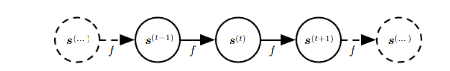
\includegraphics[width=6in]{fig/chap10/10_1.PNG} 
   \caption{这是一个展开的计算图,描述的是等式 定义的一个动态系统。每个节点代表不同时刻$t$的状态,函数$f$将$t$时刻的状态映射到$t+1$时刻的状态,每个$f$所使用的参数是一样的。}
   \label{fig:10_1}
\end{figure}

我们现在看另一个例子,我们考虑另一个动态系统,这个系统每次会接收一个外部的信号$\bm{x}^{(t)}$,
\begin{equation}
\bm{s}^{(t)} = f(\bm{s}^{(t-1)},\bm{x}^{(t)};\theta)
\label{form:10.4}
\end{equation}
我们可以看到当前状态包含所有之前时间点的历史信息。

循环神经网络可以用不同的方式来构建。我们所使用的函数几乎都可以看作是前馈神经网络(输入经过函数映射到输出),如果在函数外面再引入循环结构,那么就可以被看作循环神经网络。

很多神经网络用等式\ref{form:10.5} 或者类似式子来定义它们隐藏单元的值。为了这个状态是神经网络的隐藏单元,我们对式子\ref{form:10.4}进行了修改,用变量$h$来表示这个状态:
\begin{equation}
\bm{h}^{(t)} = f(\bm{h}^{(t-1)},\bm{x}^{(t)};\theta)
\label{form:10.5}
\end{equation}
这个式子对应的图是\ref{fig:10_2}典型的RNN会增加一个额外的结构,比如说输出层,从隐藏状态$h$中提取信息来作出预测。
\begin{figure}[htbp] %  figure placement: here, top, bottom, or page
   \centering
   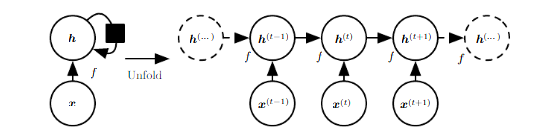
\includegraphics[width=6in]{fig/chap10/10_2.PNG} 
   \caption{一个没有输出的循环神经网络结构。网络会从输入$x$中提取信息,然后整合到隐藏状态$h$中,$h$会被传递下去作为下一个时间点输入的一部分。(左边)未展开的带环计算图。黑色的方块表示一个单位时间的延迟。(右边) 展开的计算图,本质和右边带环的图是一样的,每个节点对应一个特定的时间点。}
   \label{fig:10_2}
\end{figure}

等式\ref{form:10.5}可以用两种不同的方式来理解,我们用计算图来来帮助我们理解这两种思路。第一种可以看作是未展开的计算图,只包含有一个节点,我们甚至可以在现实中用物理实现这个模型。参考生物意义上的神经网络。在这个情况下,图中包含有一个环,它会实时的对网络进行操作。就像图\ref{fig:10_2} 左边的那个图一样。在本章中,我们在环中加了一个黑色的小方块来表示某个交互操作延后了一个时间单位,从$t$时刻的状态延后到$t+1$\footnote{译者注;这个地方不太好翻译,大家对照着图\ref{fig:10_2}去理解。}。另一种是用一个展开的计算图来描述RNN。图中有很多的节点,每个节点表示一个变量,这样每个时间点都对应一个变量来表示在那个时间点的状态。就像图\ref{fig:10_2}右边的那样。展开就是把图\ref{fig:10_2}左边带环的图映射到右边有重复结构的计算图的形式。展开的图的大小取决于序列的长度。

我们可以用函数$g^{(t)}$来表示经过$t$步展开之后的式子:
\begin{eqnarray}
\bm{h}^{(t)} & = & g^{(t)}(\bm{x}^{(t)},\bm{x}^{(t-1)},...,\bm{x}^{(2)},\bm{x}^{(1)}) \\
& = & f(\bm{h}^{(t-1)},\bm{x}^{(t)};\theta)
\end{eqnarray}

函数$g^{(t)}$把整个历史序列$(\bm{x}^{(t)},\bm{x}^{(t-1)},...,\bm{x}^{(2)},\bm{x}^{(1)})$都作为输入,输出为当前状态。但是展开的循环结构允许我们将函数用$f$来展开,我们只要递归调用函数$f$就可以得到函数$bm{h}$。展开过程有两个主要的优势:
\begin{enumerate}
\item 无论序列有多长,模型的输入变量的维度是一致的,因为从一个状态转到另一个状态的映射是固定的。而不是说把一个个长度不定的历史序列映射到一个个状态。
\item 我们每一步都可以使用一样的转换函数$f$,函数$f$的参数也可以共享。
\end{enumerate}

正因为这两个优势,我们可以只训练一个模型$f$, 这样我们不需要考虑序列的长度,每一步我们使用相同的$f$,不需要对所有可能的时间点都学习一个模型$g^{(t)}$。使用一个可以共享参数的模型能够允许我们将模型泛化到任意长度的序列中,即使某个序列的长度没有在训练集中出现。相比较不使用参数共享的模型,我们的模型在训练的时候只需要少量的训练数据。

循环图和展开图有不同的用处。循环图是简洁的。展开的计算图可以向我们展示每一步的计算,也可以展示信息流动的路径:如何沿着时间方向流动的(计算输出和损失),如何反着流动(计算梯度)。

\section{循环神经网络}
\label{sec:10.2}
在\ref{sec:10.1}我们介绍了计算图的展开和参数共享的思想。现在我们可以设计其他更复杂的递归神经网络模型。

$$\mathcal{L}$$